\chapter{คู่มือการใช้งานระบบ}
คู่มือการใช้งานทั้งหมดของแอปพลิเคชันบีอิงเวลเนส สามารถอธิบายได้ดังนี้ 

	\begin{enumerate}
			\item  หน้าจอเข้าสู่ระบบจะแสดงเมื่อสมาชิกเข้าสู่ระบบครั้งแรก ดังแสดงในรูปที่ \ref{Fig:login}
			\begin{figure}[H]
				\centering
				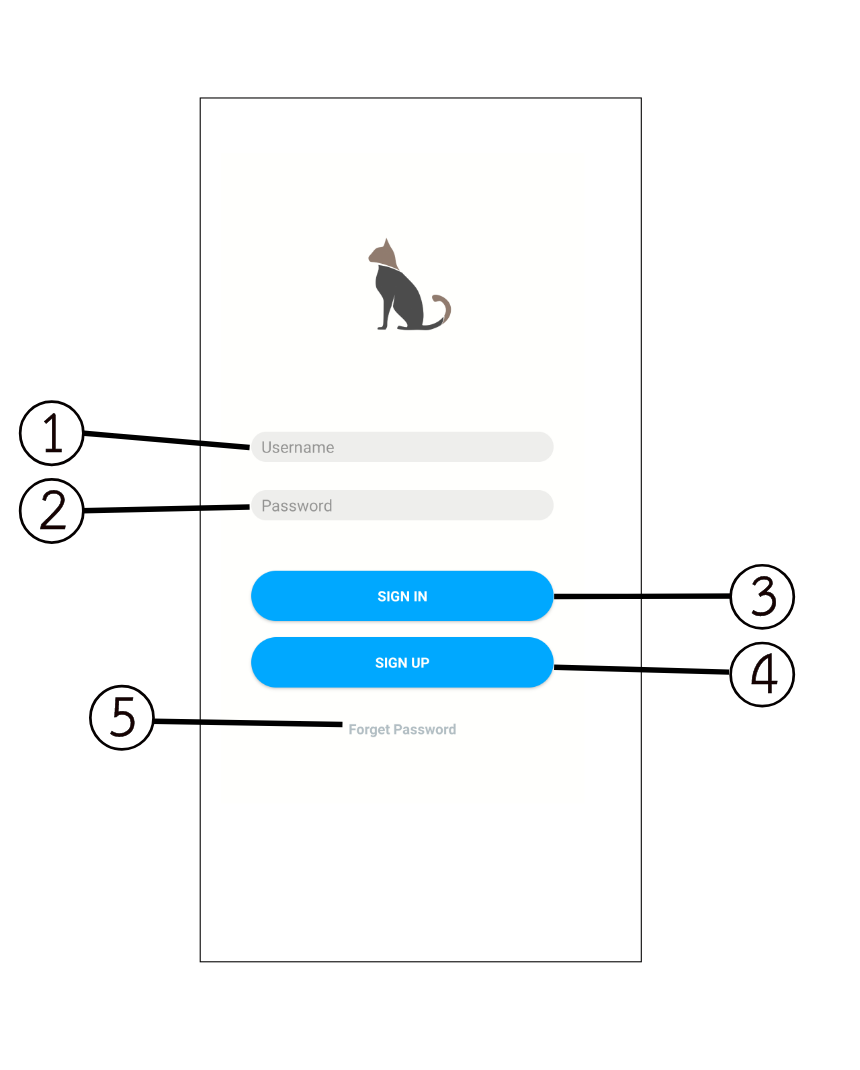
\includegraphics[width=0.5\columnwidth]{Figures/7/teach/1.png}
				\caption{หน้าจอแสดงการเข้าสู่ระบบ}
				\label{Fig:login}
			\end{figure}
		จากรูปที่ \ref{Fig:login} สามารถอธิบายการใช้งานได้ดังนี้
			\begin{itemize}[label={--}]
				\item หมายเลข 1 คือ ช่องใส่ Username
				\item หมายเลข 2 คือ ช่องใส่ Password
				\item หมายเลข 3 คือ ปุ่มสำหรับเข้าสู่ระบบ
				\item หมายเลข 4 คือ ปุ่มสำหรับสมัครสมาชิก
				\item หมายเลข 5 คือ ปุ่มสำหรับการลืมรหัสผ่าน
			\end{itemize}
		
		

			\item  หน้าจอการสมัครสมาชิกจะแสดงเมื่อทำการกดปุ่ม SIG UP ในหน้าเข้าสู่ระบบ ดังแสดงในรูปที่ \ref{Fig:Rigister}
			\begin{figure}[H]
				\centering
				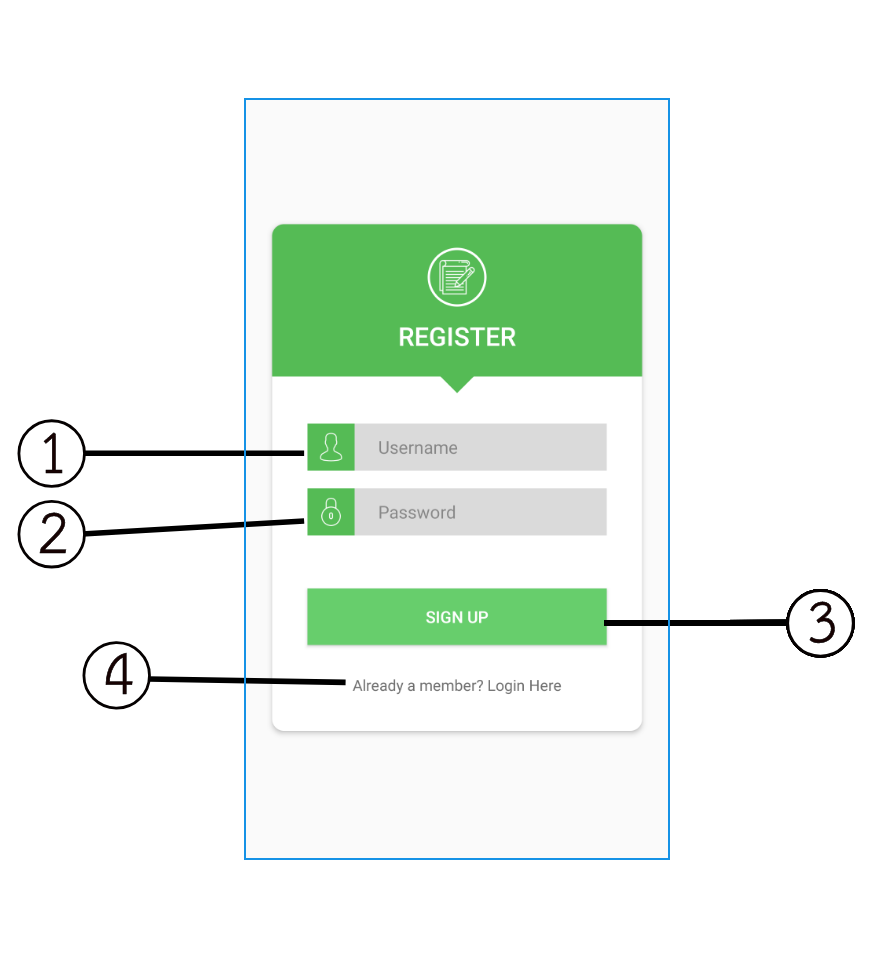
\includegraphics[width=0.5\columnwidth]{Figures/7/teach/2.png}
				\caption{หน้าจอแสดงการสมัครสมาชิก}
				\label{Fig:Rigister}
			\end{figure}
		จากรูปที่ \ref{Fig:Rigister} สามารถอธิบายการใช้งานได้ดังนี้
			\begin{itemize}[label={--}]
				\item หมายเลข 1 คือ ช่องใส่ Username
				\item หมายเลข 2 คือ ช่องใส่ Password
				\item หมายเลข 3 คือ ปุ่มสำหรับการสมัครสมาชิก
				\item หมายเลข 4 คือ ปุ่มสำหรับให้กลับไปเข้าสู่ระบบ
			\end{itemize}
			
			\item  หน้าจอแสดงการบริโภครูปแบบวัน ดังแสดงในรูปที่ \ref{Fig:Dashbord}
			\begin{figure}[H]
				\centering
				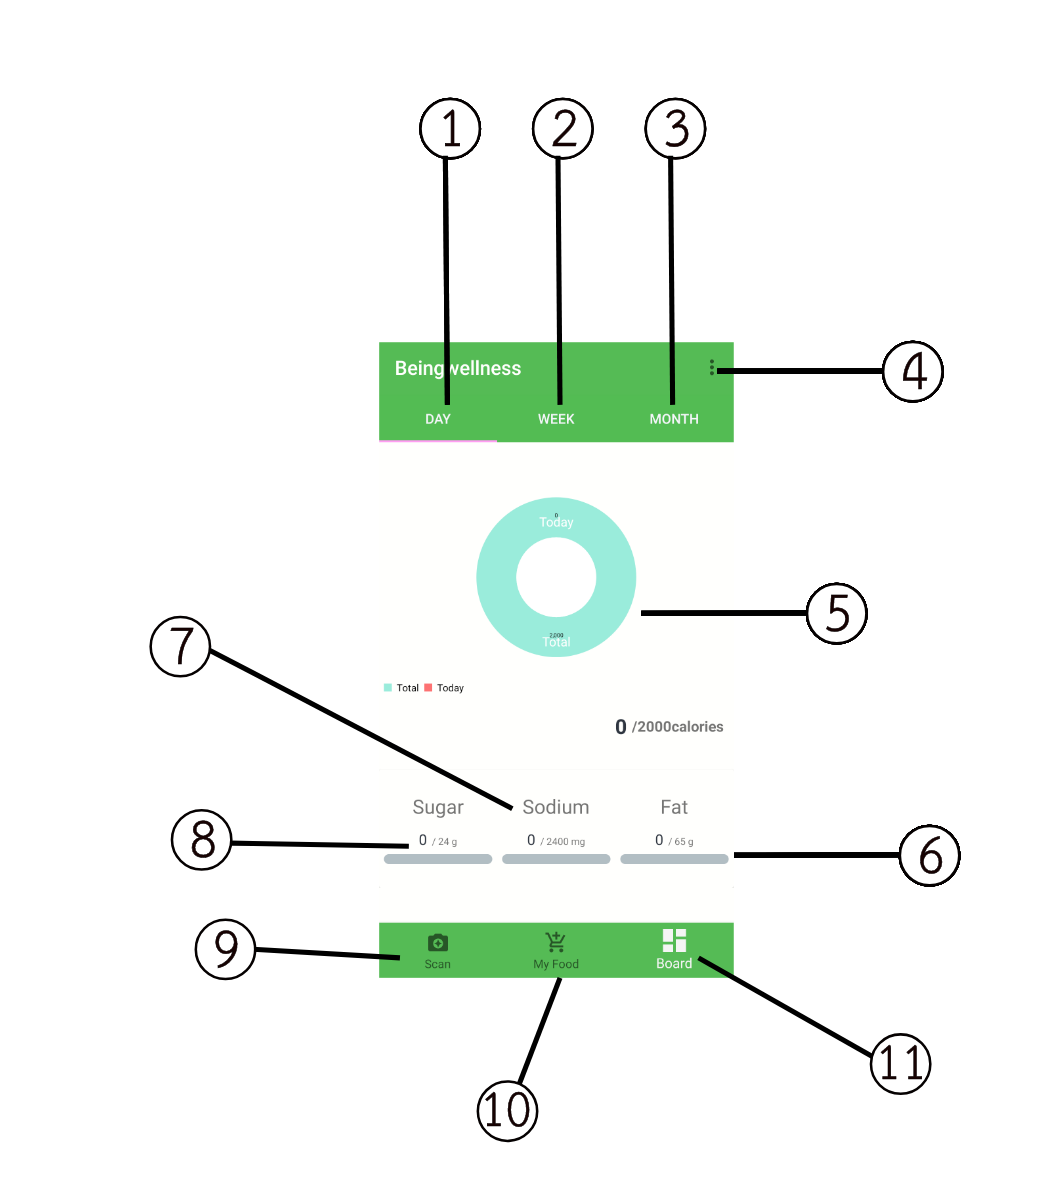
\includegraphics[width=0.5\columnwidth]{Figures/7/teach/3.png}
				\caption{หน้าจอแสดงการบริโภครูปแบบวัน}
				\label{Fig:Dashbord}
			\end{figure}
		จากรูปที่ \ref{Fig:Dashbord} สามารถอธิบายการใช้งานได้ดังนี้
			\begin{itemize}[label={--}]
				\item หมายเลข 1 คือ แถบการแสดงข้อมูลการบริโภครูปแบบวัน
				\item หมายเลข 2 คือ แถบการแสดงข้อมูลการบริโภครูปแบบสัปดาห์
				\item หมายเลข 3 คือ แถบการแสดงข้อมูลการบริโภครูปแบบเดือน
				\item หมายเลข 4 คือ ปุ่มเข้าสู่เมนูตั้งค่า
				\item หมายเลข 5 คือ Chart และตัวเลข การแสดงข้อมูลการบริโภคแคลลอรี่
				\item หมายเลข 6 คือ Progrssbar และตัวเลข การแสดงข้อมูลการบริโภคไขมัน
				\item หมายเลข 7 คือ Progrssbar และตัวเลข การแสดงข้อมูลการบริโภคโซเดียม
				\item หมายเลข 8 คือ Progrssbar และตัวเลข การแสดงข้อมูลการบริโภคน้ำตาล
				\item หมายเลข 9 คือ เมนูสแกน
				\item หมายเลข 10 คือ เมนูเพิ่มอาหาร
				\item หมายเลข 11 คือ เมนูแดชบอร์ด
			\end{itemize}


			\item  หน้าจอแสดงการบริโภครูปแบบสัปดาห์ ดังแสดงในรูปที่ \ref{Fig:week}
			\begin{figure}[H]
				\centering
				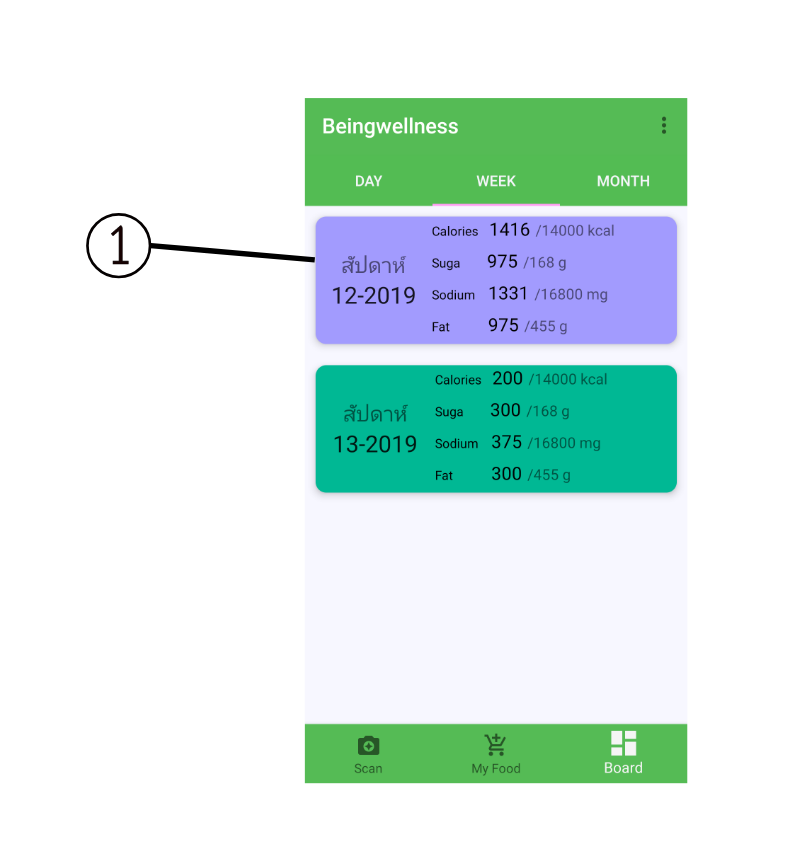
\includegraphics[width=0.5\columnwidth]{Figures/7/teach/4.png}
				\caption{หน้าจอแสดงการบริโภครูปแบบสัปดาห์}
				\label{Fig:week}
			\end{figure}
		จากรูปที่ \ref{Fig:week} สามารถอธิบายการใช้งานได้ดังนี้
			\begin{itemize}[label={--}]
				\item หมายเลข 1 คือ รายการอาหารและข้อมูลการบริโภครูปแบบสัปดาห์
				\end{itemize}
			
				\item  หน้าจอแสดงการบริโภครูปแบบเดือน ดังแสดงในรูปที่ \ref{Fig:Month}
				\begin{figure}[H]
					\centering
					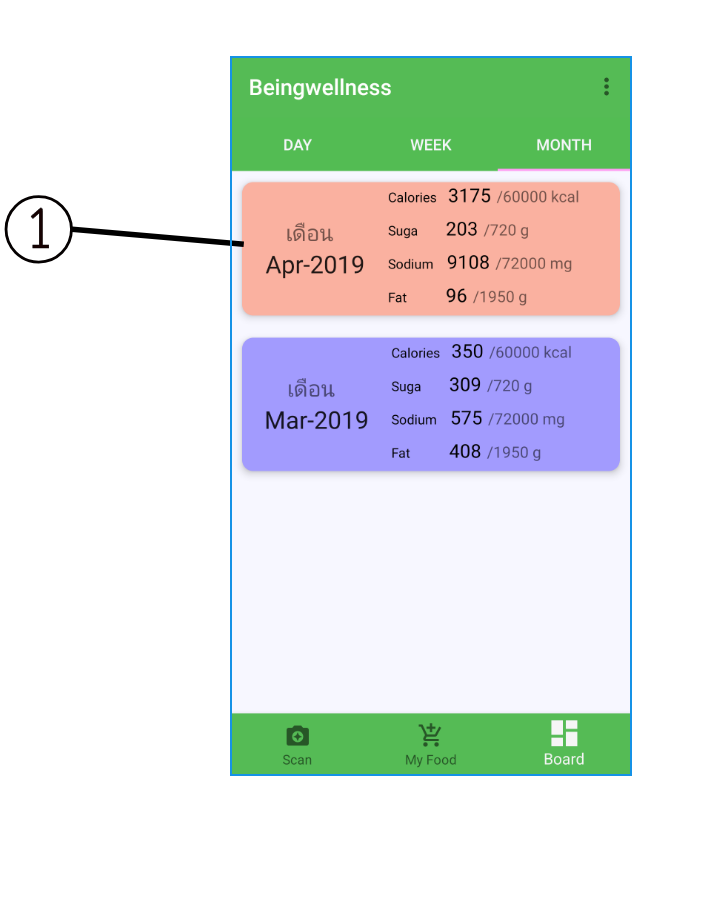
\includegraphics[width=0.5\columnwidth]{Figures/7/teach/5.png}
					\caption{หน้าจอแสดงการบริโภครูปแบบเดือน}
					\label{Fig:Month}
				\end{figure}
			จากรูปที่ \ref{Fig:Month} สามารถอธิบายการใช้งานได้ดังนี้
				\begin{itemize}[label={--}]
					\item หมายเลข 1 คือ รายการอาหารและข้อมูลการบริโภครูปแบบสัปดาห์
					\end{itemize}
			
					\item  หน้าจอแสดงสแกนอาหาร ดังแสดงในรูปที่ \ref{Fig:scan}
					\begin{figure}[H]
						\centering
						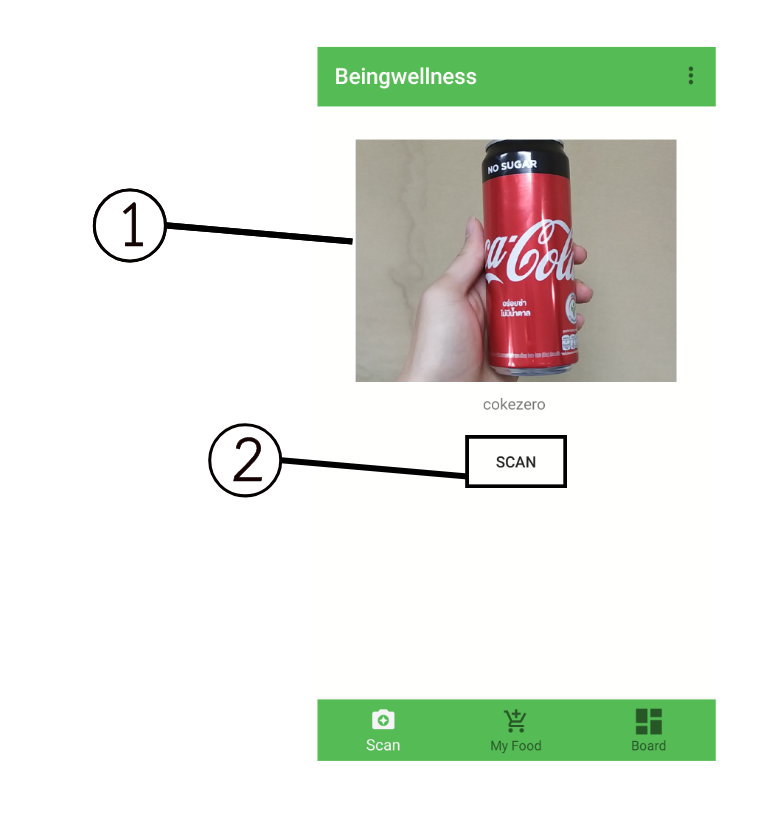
\includegraphics[width=0.5\columnwidth]{Figures/7/teach/7.png}
						\caption{หน้าจอแสดงสแกนอาหาร}
						\label{Fig:scan}
					\end{figure}
				จากรูปที่ \ref{Fig:scan} สามารถอธิบายการใช้งานได้ดังนี้
					\begin{itemize}[label={--}]
						\item หมายเลข 1 คือ กล้องที่จะทำการสแกน
						\item หมายเลข 2 คือ ปุ่มสแกน
						\end{itemize}

						\item  หน้าจอแสดงข้อมูลอาหาร ดังแสดงในรูปที่ \ref{Fig:food}
					\begin{figure}[H]
						\centering
						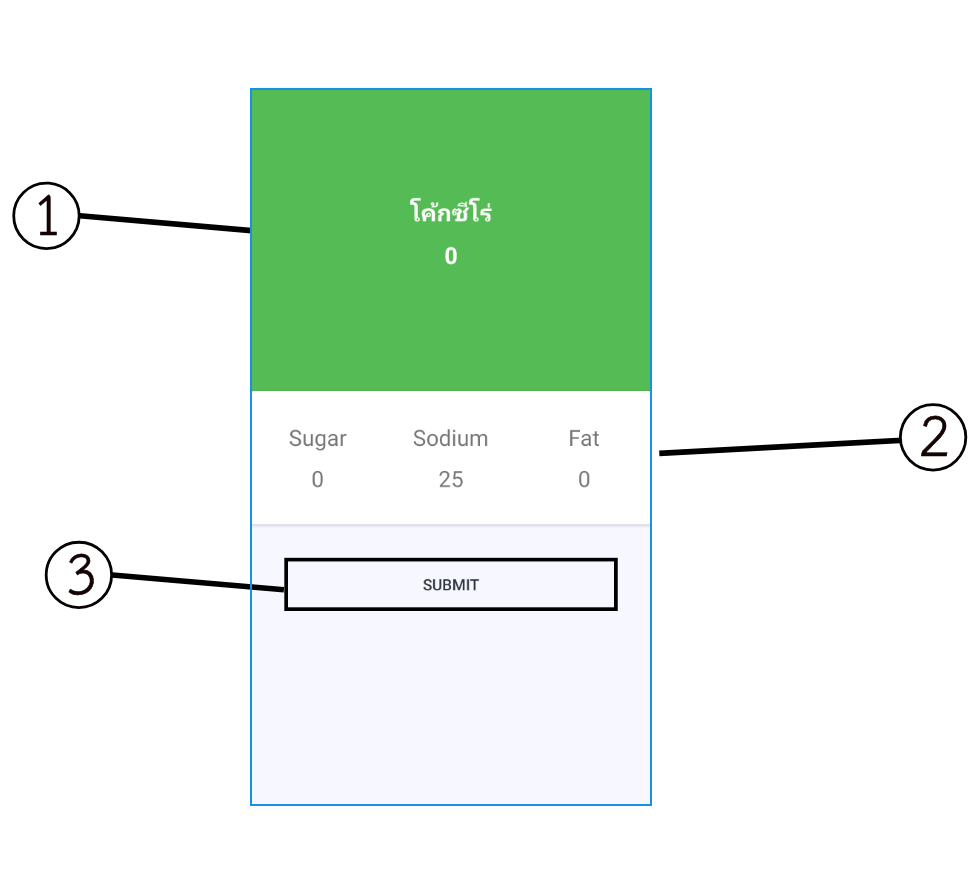
\includegraphics[width=0.5\columnwidth]{Figures/7/teach/6.png}
						\caption{หน้าจอแสดงสแกนอาหาร}
						\label{Fig:food}
					\end{figure}
				จากรูปที่ \ref{Fig:food} สามารถอธิบายการใช้งานได้ดังนี้
					\begin{itemize}[label={--}]
						\item หมายเลข 1 คือ ส่วนแสดงข้อมูลอาหารได้แก่ ชื่ออาหารและแคลลอรี่
						\item หมายเลข 2 คือ ส่วนแสดงข้อมูลอาหารได้แก่ น้ำตาล โซเดียม ไขมัน
						\item หมายเลข 3 คือ ปุ่มทำการบันทึกข้อมูลอาหาร
						\end{itemize}




						\item  หน้าจอแสดงการเปลี่ยน E-mail และ Password ดังแสดงในรูปที่ \ref{Fig:change}
						\begin{figure}[H]
							\centering
							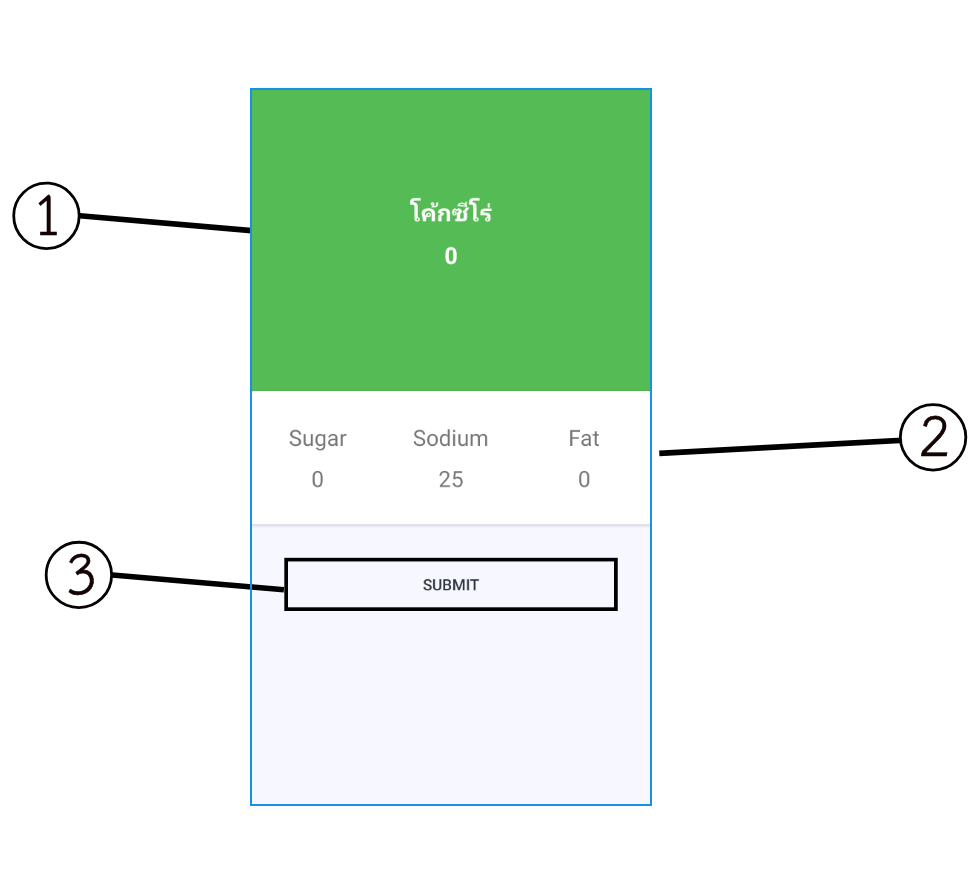
\includegraphics[width=0.5\columnwidth]{Figures/7/teach/6.png}
							\caption{หน้าจอแสดงสแกนอาหาร}
							\label{Fig:change}
						\end{figure}
					จากรูปที่ \ref{Fig:change} สามารถอธิบายการใช้งานได้ดังนี้
						\begin{itemize}[label={--}]
							\item หมายเลข 1 คือ ส่วนที่ใส่่ E-mail หรือ Password
							\item หมายเลข 2 คือ ปุ่มทำการยืนยัน
							\end{itemize}
							
							\item  หน้าจอแสดงการลบผู้ใช้ \ref{Fig:del}
							\begin{figure}[H]
								\centering
								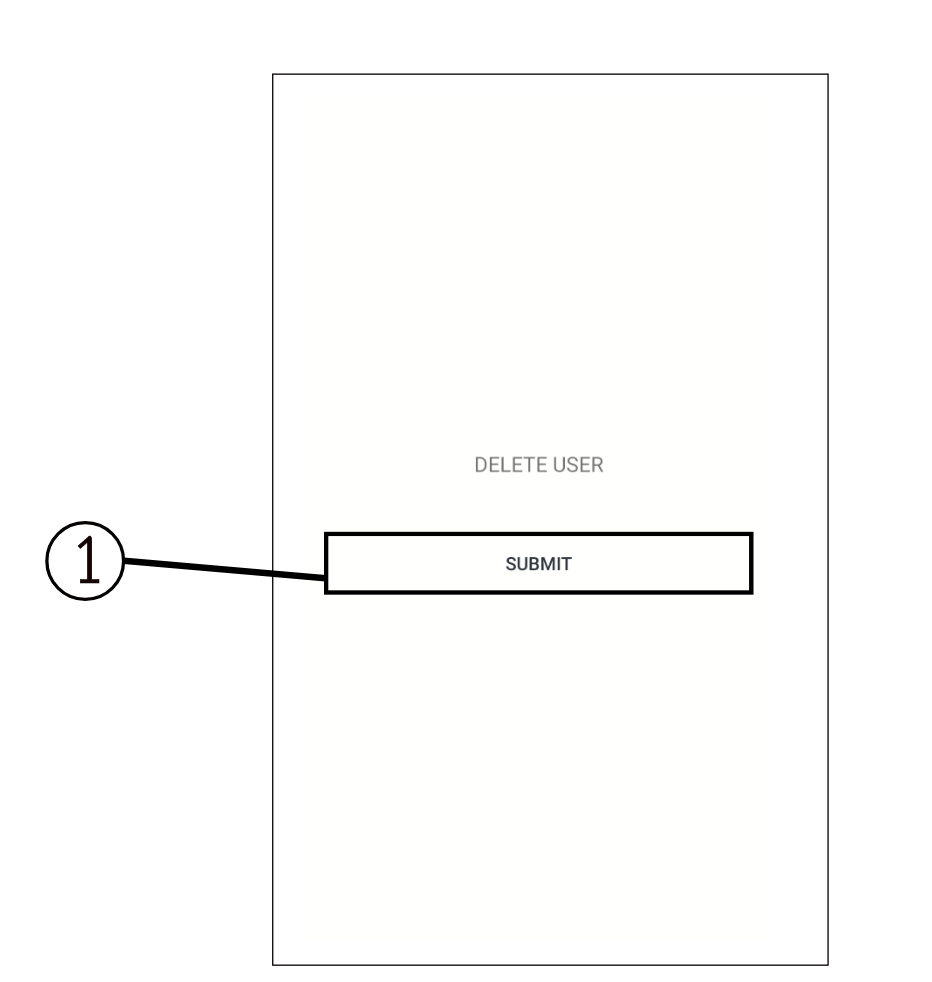
\includegraphics[width=0.5\columnwidth]{Figures/7/teach/10.png}
								\caption{หน้าจอแสดงสแกนอาหาร}
								\label{Fig:del}
							\end{figure}
						จากรูปที่ \ref{Fig:del} สามารถอธิบายการใช้งานได้ดังนี้
							\begin{itemize}[label={--}]
								\item หมายเลข 1 คือ ปุ่มทำการลบสมาชิก
								\end{itemize}


								\item  หน้าจอรายการอาหารที่เพิ่ม \ref{Fig:useradd}
								\begin{figure}[H]
									\centering
									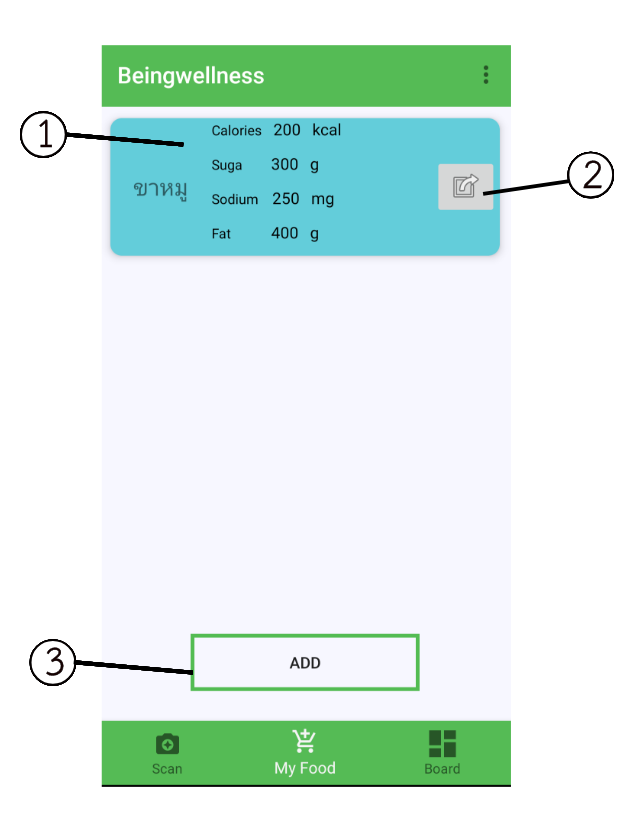
\includegraphics[width=0.5\columnwidth]{Figures/7/teach/13.png}
									\caption{หน้าจอรายการอาหารที่เพิ่ม}
									\label{Fig:useradd}
								\end{figure}
								จากรูปที่ \ref{Fig:useradd} สามารถอธิบายการใช้งานได้ดังนี้
								\begin{itemize}[label={--}]
									\item หมายเลข 1 คือ รายการอาหารที่เพิ่ม
									\item หมายเลข 2 คือ ปุ่มสำหรับบันทึกข้อมูลอาหาร
									\item หมายเลข 3 คือ ปุ่มสำหรับเพิ่มอาหาร
								
									\end{itemize}


									\item  หน้าจอเพิ่มอาหาร \ref{Fig:addbyuse}
									\begin{figure}[H]
										\centering
										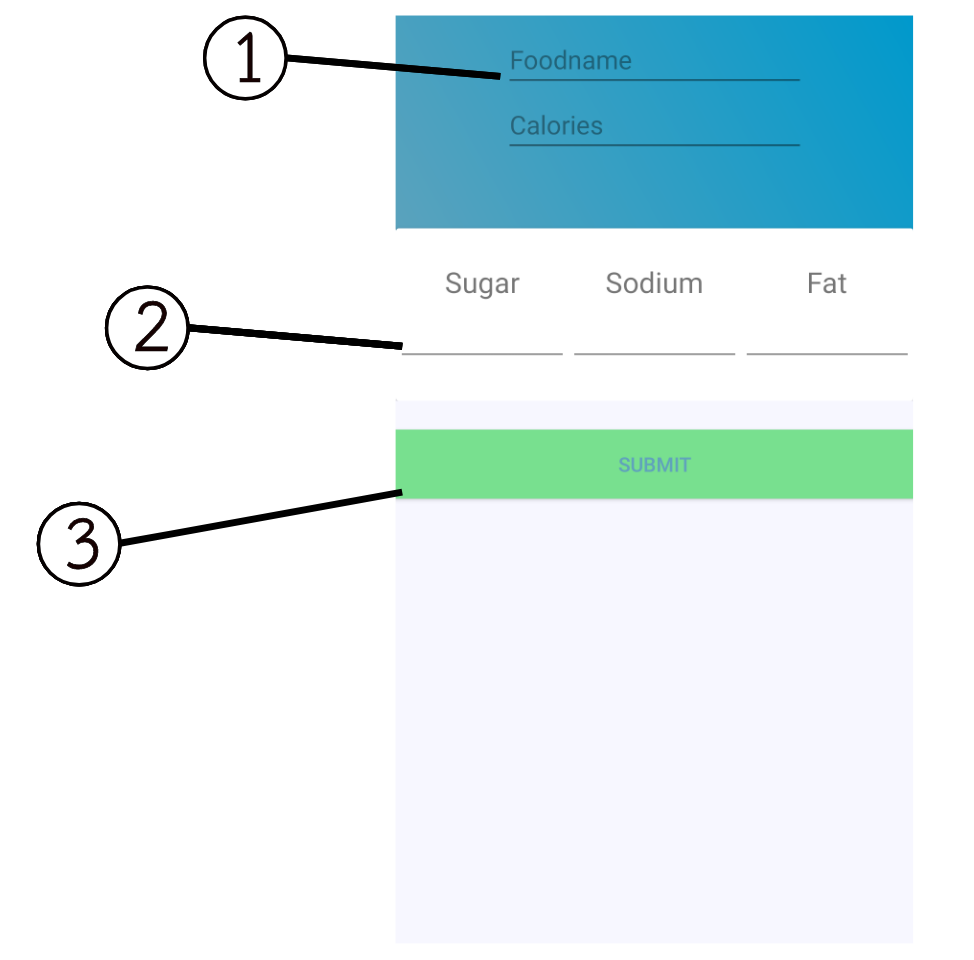
\includegraphics[width=0.5\columnwidth]{Figures/7/teach/11.png}
										\caption{หน้าจอเพิ่มอาหาร}
										\label{Fig:addbyuse}
									\end{figure}
									จากรูปที่ \ref{Fig:addbyuse} สามารถอธิบายการใช้งานได้ดังนี้
									\begin{itemize}[label={--}]
										\item หมายเลข 1 คือ ส่วนของการเพิ่มชื่ออาหารและเเคลลอรี่
										\item หมายเลข 2 คือ ส่วนของการเพิ่ม น้ำตาล โซเดียม ไขมัน
										\item หมายเลข 3 คือ ปุ่มสำหรับเพิ่มอาหาร
									
										\end{itemize}


									\item  หน้าจออัพเดทอาหารที่เพิ่ม \ref{Fig:upfood}
									\begin{figure}[H]
										\centering
										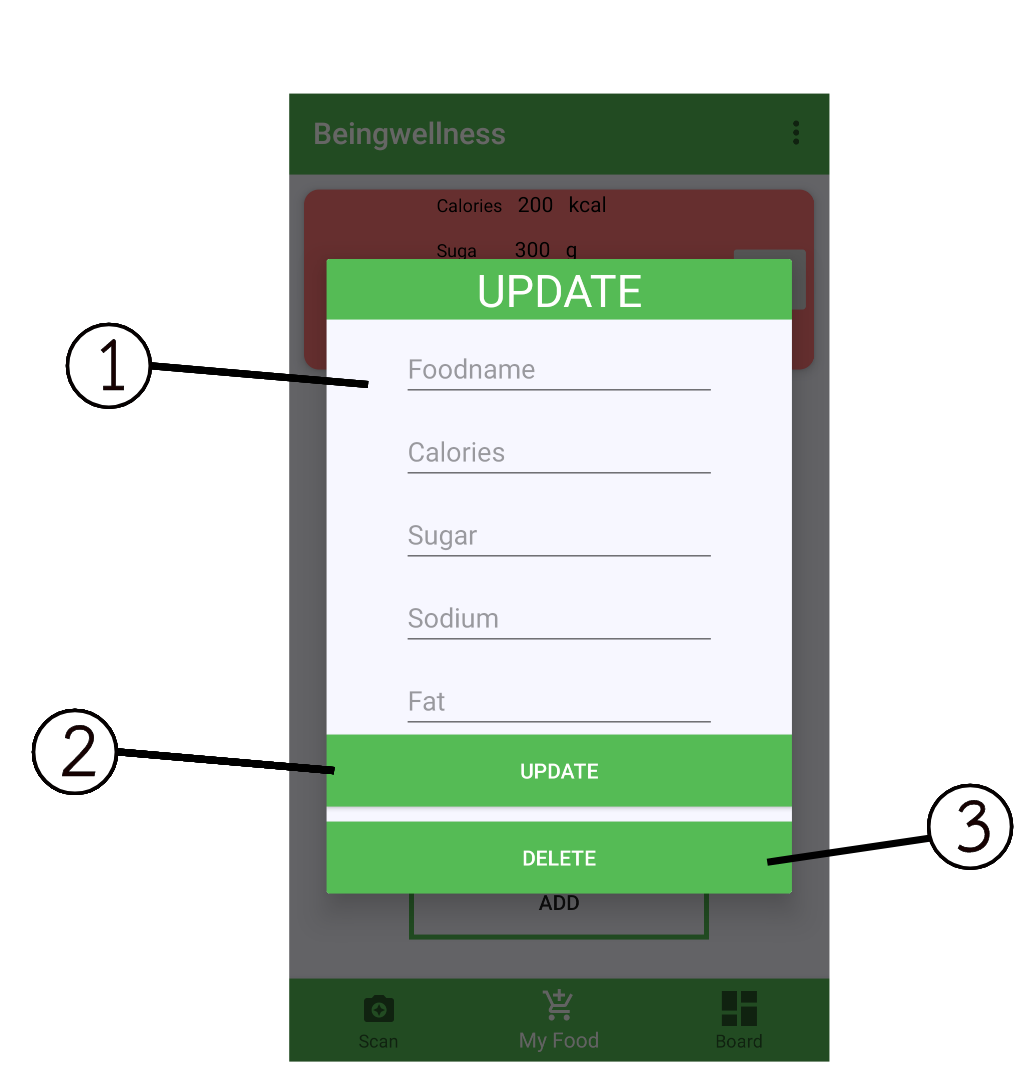
\includegraphics[width=0.5\columnwidth]{Figures/7/teach/12.png}
										\caption{หน้าจออัพเดทอาหารที่เพิ่ม}
										\label{Fig:upfood}
									\end{figure}
									จากรูปที่ \ref{Fig:upfood} สามารถอธิบายการใช้งานได้ดังนี้
									\begin{itemize}[label={--}]
										\item หมายเลข 1 คือ ส่วนของการอัพเดท ชื่ออาหาร แคลลอรี่  น้ำตาล โซเดียมและไขมัน
										\item หมายเลข 2 คือ  ปุ่มอัพเดท
										\item หมายเลข 3 คือ ปุ่มลบอาหาร
									
										\end{itemize}
	\end{enumerate}
				
